\section{Introduction}
\subsection{Système de développement}

Dans le cadre de ce projet, la correction a été réalisée sur un poste Linux\footnote{Ici, Ubuntu 14.04 LTS - 64 bits}. Ainsi, nous avons pu nous servir des outils tels que \textit{Valgrind} ou \textit{FlawFinder}.\\
Les fonctions propres à \textit{Microsoft} telles que \textit{strcpy\_s} n'ont ainsi pas été utilisées.

\subsection{Le code initial}

Dans un premier temps, il est nécessaire d'analyser le code original :
\begin{lstlisting}[language=C]
/* --------------------------------------------------------- */
/* Objectif : Corriger les erreurs statiques et dynamiques   */
/*            de ce programme                                */
/* --------------------------------------------------------- */

int main(int argc, char *argv[])
{
    /* On ne touche pas a la variable "size" */
    int size = 16;
    int length = 0;
    char * buf;
	
    printf(argv[1]);
	
    buf = (char*)malloc(sizeof(char)*size + 1);
	
    strcpy_s(buf, sizeof(buf), argv[2]);
    printf("buffer : %s\n", buf);
	
    /* ----------------------------------------------------- */
    /* On ne touche pas au contenu "testdubuffer"            */
    /* mais on peut creer une variable reprenant ce contenu  */
    /* ----------------------------------------------------- */
	
    strcpy_s(buf, sizeof(buf), "testdubuffer");
	
    length = strlen(buf);
    if(length != 0)
        printf("buffer : %s\n", buf);
    else
        free(buf);
		
    return 0;
}
\end{lstlisting}
\subsection{Compilation du code}
Afin de compiler ce code, nous remplacerons la fonction \textit{strcpy\_s} par la fonction \textit{strcpy}.\\
Cependant, nous pouvons remarquer que ce code, ici écrit sous Visual Studio, ne réagis pas de la même façons une fois exécuté sous Windows. En effet, celui-ci va nous permettre de n'afficher que \enquote{\textit{testdubu}}. Cela est du à l'argument donnée à la fonction \textit{strcpy\_s} : \textit{sizeof(buf)}. Ce dernier va alors faire une copie d'une taille de 8 octets (taille du pointeur). Ainsi, le fonctionnement basique du code est légèrement différent.\\~\\
Nous utiliserons ensuite le fichier \textit{Makefile} suivant afin de compiler le programme :
\newpage
\begin{lstlisting}[language=make]
CC=gcc
CFLAGS=-W -Wall -ansi 
EXEC=DynStat_old

all: $(EXEC)

DynStat_old: DynStat_old.o
	$(CC) -o DynStat_old DynStat_old.o

DynStat.o_old: DynStat_old.c
	$(CC) -o DynStat_old.o -c DynStat_old.c

clean:
	rm -rf *.o
\end{lstlisting}
Lors de la première compilation, il est possible de se rendre compte que nous avons premièrement des \textit{warning} :
\begin{figure}[H]
  \centering
  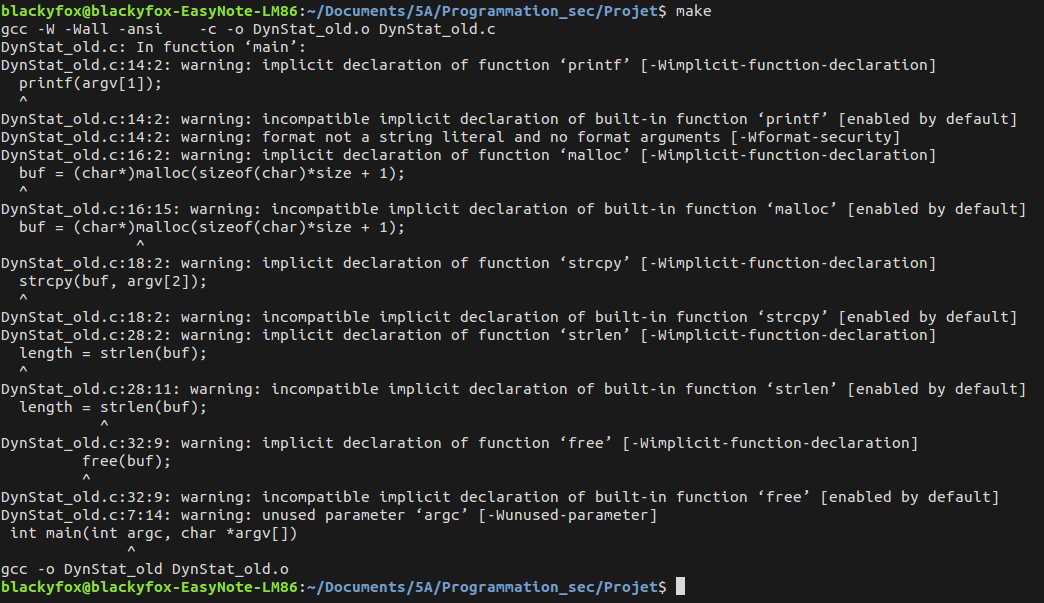
\includegraphics[width=.9\textwidth]{img/compile1.png}
  \caption{Première compilation du programme}
  \label{img:1}
\end{figure}
Ces erreurs sont du au fait que notre code n'a aucune bibliothèque d'incluse. Ainsi les fonctions utilisées, même les plus courantes comme \textit{printf}, ne sont pas reconnues. Pour palier à cela, nous allons inclure trois bibliothèques :
\begin{lstlisting}
#include <stdio.h>
#include <string.h>
#include <stdlib.h>
\end{lstlisting}
Grâce à ces dernières, nous allons avoir accès à de nombreuses fonctions pour la gestion de chaînes de caractères, l'allocation dynamique de la mémoire, etc\ldots\\
Nous pouvons alors recompiler le programme et obtenir la sortie suivante :
\begin{figure}[H]
  \centering
  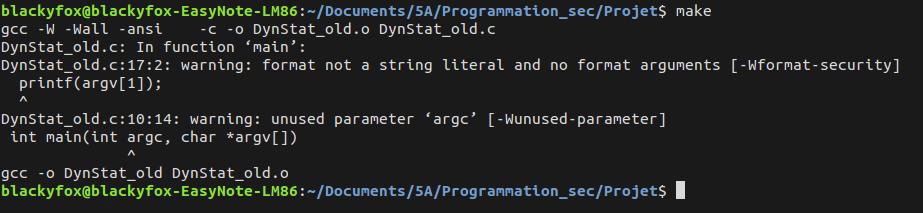
\includegraphics[width=.9\textwidth]{img/compile2.png}
  \caption{Seconde compilation du programme}
  \label{img:2}
\end{figure}
Malgré les \textit{warnings}, un fichier exécutable a été créé. Nous pouvons alors tester le programme.\\
\subsection{Exécution du code}\label{sec:exe}
En l'exécutant sans aucun argument donné, nous obtenons la sortie suivante :
\begin{figure}[H]
  \centering
  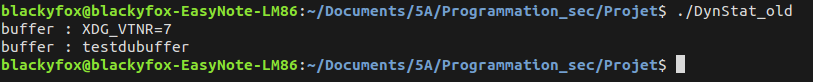
\includegraphics[width=.9\textwidth]{img/exe1.png}
  \caption{Première exécution du programme}
  \label{img:3}
\end{figure}
On se rend alors compte que nous avons déjà ici des erreurs. En effet, en lisant le code, nous pouvons voir que le programme récupère deux chaînes de caractères données en arguments. Ici, bien qu'aucun argument n'ai été donné, le programme s'exécute. On peut aussi remarquer sur la première ligne de la sortie (c.f. figure \ref{img3}) que le programme affiche une valeur. Cette dernière, censée être le second argument donné, est en réalité une variable d'environnement du système.\\
En donnant un argument au programme nous obtenons le résultat suivant :
\begin{figure}[H]
  \centering
  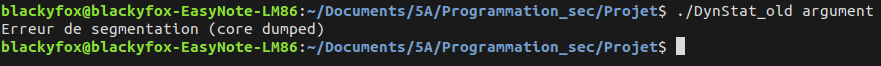
\includegraphics[width=.9\textwidth]{img/exe2.png}
  \caption{Seconde exécution du programme}
  \label{img:4}
\end{figure}
Ici, nous avons une erreur de segmentation.\\
Nous pouvons utiliser l'outil \textit{Valgrind} afin de comprendre un peu plus pourquoi nous avons eu cette erreur :
\begin{figure}[H]
  \centering
  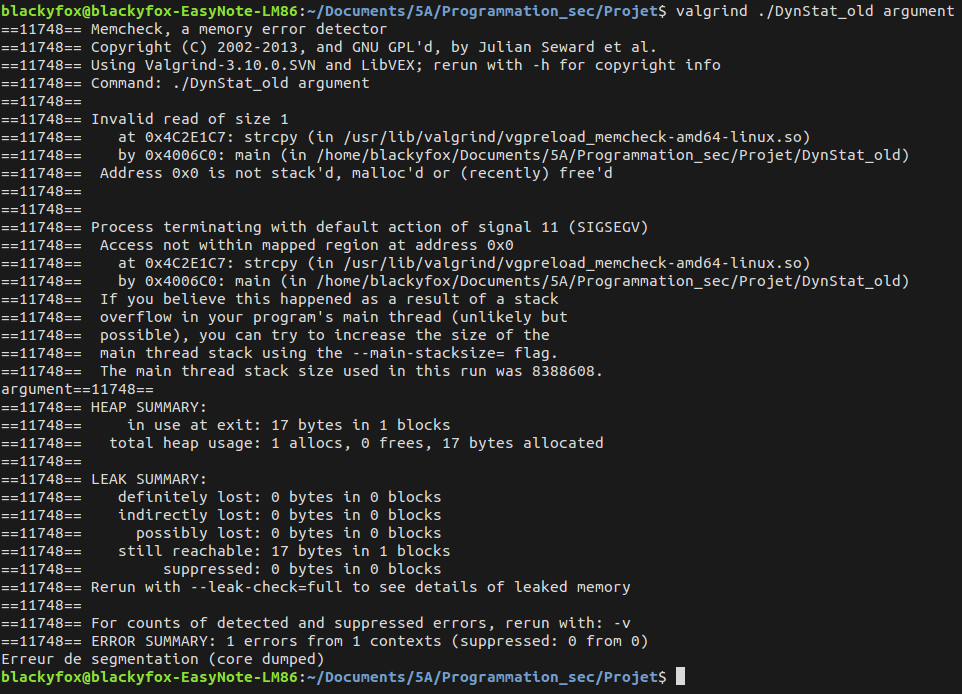
\includegraphics[width=.9\textwidth]{img/valg1.png}
  \caption{Seconde exécution du programme avec \textit{Valgrind}}
  \label{img:5}
\end{figure}
Ainsi, nous pouvons voir que le programme a essayé de lire un espace mémoire qui ne lui était pas réservé.\\
Nous savons donc que nous devrons faire attention au nombre d'arguments donnés au programme lors de la correction.\\
Enfin, en donnant deux arguments au programme nous obtenons la sortie suivante :
\begin{figure}[H]
  \centering
  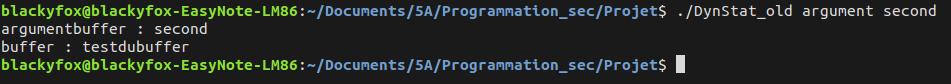
\includegraphics[width=.9\textwidth]{img/exe3.png}
  \caption{Troisième exécution du programme}
  \label{img:6}
\end{figure}
Dans ce cas, nous pouvons voir que le programme réalise bien ce qu'il lui a été demandé :
\begin{enumerate}
 \item Afficher le premier argument
 \item Afficher \enquote{buffer : } suivi du contenu de la variable \textit{buf}, contenant le second argument
 \item Afficher \enquote{buffer : } suivi du contenu de la variable \textit{buf}, contenant la chaîne \enquote{testdubuffer}
\end{enumerate}
Si nous donnons des arguments supplémentaires au programme, nous voyons que ce dernier ne traite pas ces arguments :
\begin{figure}[H]
  \centering
  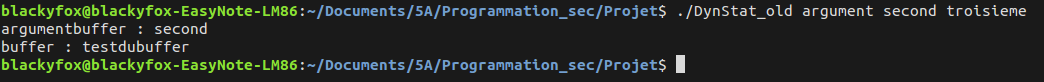
\includegraphics[width=.9\textwidth]{img/exe4.png}
  \caption{Quatrième exécution du programme}
  \label{img:7}
\end{figure}